\renewcommand{\cleardoublepage}{}
\renewcommand{\clearpage}{}

\section{Fermion Masses in the Standard Model and Quark Mixing}
\label{Chap_1_Sec_3}

As referenced previously, given the charges of the fermion and lepton fields we cannot construct a gauge invariant theory with explicit mass terms for fermions. 
%
The mass of these particles are generated through the Higgs mechanism, via Yukawa terms between the fermions and the scalar field. 
%
These interactions can be seen in Eq\,(\ref{eq:Yukawa2}), 
%
\begin{equation} 
\label{eq:Yukawa2}
\mathcal{L}_{Yuk} = Y^u_{ij} \bar{Q}_{L_i} u_{R_j}  \tilde{H} + Y^d_{ij} \bar{Q}_{L_i}  d_{R_j} H  + Y^e_{ij} \bar{L}_{L_i}  e_{R_i} H + \text{H.c.} , 
\end{equation} 
%
as the Higgs field settles into the EW VEV (see Eq.\,(\ref{shame})) mass terms for the quarks and leptons are generated. 
%
The Higgs mechanism generates the mass for all the fermionic and leptonic particles except for neutrinos, this is due to the SM not containing right handed neutrinos, i.e it is impossible build terms that would lead to neutrino masses without explicitly breaking the SM symmetry group.
% 
The addition of right handed neutrino fields is very commonly made in BSM scenarios. 

To reach the physical states from the weak eigenbasis we must diagonalize the Yukawa matrices. This is done through bi-unitary transformations. 
% 
We can write these transformation under the form,
%
\begin{equation}
\label{YukawaMasses} 
M^{u,d,e}_{\text{diag.}}= U^{u,d}_L Y^{u,d} U^{u,d}_R \frac{v}{\sqrt{2}} , 
\end{equation} 
%
where $U^{u,d}_L$ and $U^{u,d}_R$ are the required 4 unitary matrices. 

%{\color{gray} The charged lepton Yukawa matrix can always be made real and positive through a bi-unitarity transformation.  
%
%Meaning the Yukawa matrix for the leptons contains only 3 real physical parameters that correspond to the Lepton masses. } 
%
For simplicity sake we assume that the leptonic Yukawa couplings matrix $Y^{e}$ is flavour diagonal i.e. a diagonal matrix needing not to be transformed. This makes only the quarks to be relevant to our discussion.  

Naturally, we can invert Eq.\,(\ref{YukawaMasses}), returning, 
\begin{equation}
\label{eq:YukawaBiUni}
%\begin{split}
Y^u_{ij} = \frac{\sqrt{2}}{v} (U_L^u M^u_{\text{diag.}} U_R^u)_{ij} \quad , \quad Y^d_{ij} = \frac{\sqrt{2}}{v} (U_L^d M^d_{\text{diag.}} U_R^d)_{ij} . 
%\end{split}
\end{equation}
%
Considering the Higgs mechanism, we can see this change creates mass terms for physical quark fields by replacing the result of Eq.\,(\ref{eq:YukawaBiUni}) in the Yukawa portion of the Lagrangian (Eq.\,(\ref{eq:YukawaSM})).
%
\begin{gather}
\mathcal{L}_{Yuk} \supset 
- \frac{v}{\sqrt{2}} Y^d_{ij} \begin{pmatrix} \overline{u}_{L\,i} & \overline{d}_{L\,i}  \end{pmatrix}  d_{R\,j} \tilde{H}
%
-\frac{v}{\sqrt{2}} Y^u_{ij} \begin{pmatrix} \overline{u}_{L\,i} & \overline{d}_{L\,i}  \end{pmatrix} \, u_{R\,j} + \text{H.c.} \nonumber  \\ 
% % % 
 \Downarrow \nonumber \\
-(U_L^d M^d_{\text{diag.}} U_R^d)_{ij} d_{L\,i} \, d_{R\,j}  - (U_L^u M^u_{\text{diag.}} U_R^u)_{ij} u_{L\,i} \, u_{R\,j} + \big(\text{Interactions with } h\big) + \text{H.c.} \\ 
 \Downarrow  \nonumber \\ 
-M^d_{\text{diag.}_j} d_{L\,i}^\prime \, d_{R\,j}^\prime  - M^u_{\text{diag.}_j} u_{L\,i}^\prime \, u_{R\,j}^\prime + \big(\text{Interactions with }h\big) + \text{H.c.}  \nonumber  
\end{gather}
%
where the primed fields are the quark fields in the mass basis, defined as, 
\begin{equation}
\begin{split}
d^\prime_{L,R} = U^d_{L,R} d_{L,R}, \\
u^\prime_{L,R} = U^u_{L,R} u_{L,R}. 
\end{split}  
\end{equation}
% 
Note that the increasing masses seen in each generation depend directly on the  hierarchy of the Yukawa terms. This means that the mass of all particles directly relates to how strongly they each interact with the Higgs boson.
%
If you then take into account the real masses e.g. for the leptons, the tau mass is in the GeV range while the electron's is in the 0.1 MeV range. This translate to very different couplings for each flavour. 
%
This hierarchy is unjustified in the SM. 

As a result of this redefinition we can now look at the gauge interactions to see that charged currents appear where $W^\pm$ couples to the physical $u^\prime_{L_j}$ and $d^\prime_{L_j}$ quarks. 
%
The coupling of the fermions to the gauge fields changes by virtue of the fact that only left handed quarks are $\mathrm{SU(2)_L}$ doublets. If we expand the up and down quark fields on the kinetic portion of the Lagrangian,
%
\begin{equation}
\label{LagFermFCCCs}
\begin{aligned}
\mathcal{L}_{ferm} \supset & 
\frac{1}{2} \bar{u}^\prime_L \gamma^\mu \left( g^\prime Y B_\mu + g Z_\mu  \right) \left(U^u_L U^{u \dagger}_L \right) u^\prime_L - \frac{1}{\sqrt{2}} g \bar{u}^\prime_L \gamma^\mu \left( U^u_L U^{d \dagger}_L \right) d^\prime_L W^+_\mu \\    
- 
& \frac{1}{\sqrt{2}} g \bar{d}^\prime_L \gamma^\mu \left( U^u_L U^{d \dagger}_L \right) u^\prime_L W^-_\mu 
+ 
\frac{1}{2} \bar{d}^\prime_L \gamma^\mu \left( g^\prime Y B_\mu - g Z_\mu \right) \left( U^d_L U^{d \dagger}_L \right) d^\prime_L \quad , 
\end{aligned}
\end{equation}
%
By employing properties of unitary matrices, namely, $ \mathrm{U}^{u,d}_{L,R} \mathrm{U}^{u,d \dagger}_{L,R} = 1$, we note that the interactions with the neutral bosons remain the same in the mass basis.
%
However the charged currents are affected by this change.
%
Therefore, we define the Cabibbo-Kobayashi-Maskawa (CKM) matrix, as $V_{CKM} = U^u_L U^{u ^\dagger }_R $ and write the sensitive terms,
%
\begin{equation}
\mathcal{L}_{kin} \supset \frac{1}{\sqrt{2}} g \overline{u}^\prime_L \gamma^\mu V_{CKM} d_L^\prime W^+_\mu + \text{H.c.} \quad , 
\end{equation}
%
The CKM matrix, is a $3 \times 3$ unitary matrix. It is a parametrization of the three mixing angles and a CP-violating KM (Kobayashi-Maskawa) phase. % There are many possible conventions to represent the CKM matrix.
%
The mixing angles refer to those between the up and down quark families. We can see their hierarchy in Fig. \ref{fig:QuarkCKM}.

It is through this complex phase in the CKM matrix that the SM can account for the phenomena of $\mathcal{CP}$ violation.
%
First observed in the famous $K^0$ decay into $\mu^+$ $\mu^-$ ($CP=+1$ and $CP=-1$ respectively) \cite{PhysRevLett.13.138}, that won the 1980 Nobel Prize \cite{NobelPrize:1980-Physics}. 
%
The discovery opened the door to questions still at the core of particle physics and of cosmology today.
%
Not just the lack of an exact CP-symmetry, but also the fact that it is so close to a symmetry.

\begin{figure}[H]
	\centering
	\vspace{1em}
   \begin{fmffile}{feyngraph_box}
   \begin{fmfgraph*}(175,60)
   \fmfstraight
   \fmfleft{i2,K,i1}
   \fmfright{o2,o1}
%    % quarks
   \fmf{fermion}{i1,t1}
    \fmf{fermion}{t4,i2}
    \fmflabel{d}{i1}
    \fmflabel{$\overline{\text{s}}$}{i2}
    \fmfv{l.d=65,l.a=180,l={$\text{K}^0$\mylbrace{76}{0}}}{K}
    % placeholders quarks-muons
    \fmf{phantom,tension=1}{t1,t2}
    \fmf{phantom,tension=1}{t4,t3}
%    % muons
    \fmf{fermion,tension=1}{t2,o1}
    \fmf{fermion,tension=1}{o2,t3}
    \fmflabel{$\mu^-$}{o1}
    \fmflabel{$\mu^+$}{o2}
%    % box loop
    \fmf{boson,tension=0,label=$\text{W}^-$,label.side=left}{t1,t2}
    \fmf{boson,tension=0,label=$\text{W}^+$,label.side=left}{t3,t4}
    \fmf{fermion,tension=0,label=u}{t1,t4}
    \fmf{fermion,tension=0,label=$\nu_\mu$}{t3,t2}
    \fmfv{d.shape=circle,d.size=4,l=$\sin(\theta_{\mathrm{C}})\quad$,l.a=110}{t1}
    \fmfv{d.shape=circle,d.size=4,l=$\cos(\theta_{\mathrm{C}})\quad$,l.a=-110}{t4}
    \fmfv{d.shape=circle,d.size=4}{t1}
    \fmfv{d.shape=circle,d.size=4}{t4}
    \end{fmfgraph*}
    \end{fmffile}
\vspace{1em}
	\caption{Box diagram describing $K_L^0\rightarrow\mu^-\mu^+$, through an intermediate $u$ quark. }
	\label{fig:Kaon}
\end{figure}
%
We avoided discussing leptons since in the SM their mass eigenstates can be easily shown to have no real consequence besides a change of basis. 
%
We might also note a very interesting feature of the Standard Model, by consequence of the $\mathrm{SU(2)_L \times U(1)_Y }$ symmetry we can see that in Eq.(\ref{LagFermFCCCs}) there are no interactions of the right handed unitary matrices and thus no mixing, coupling, or charged currents of right handed quarks, making them theoretically invisible. % to measurements.  
%
The nature of CKM elements and how the quarks behavior differs when interacting weakly trough neutral currents can be seen in the following figure,
%
\begin{figure}[H]
	\centering
	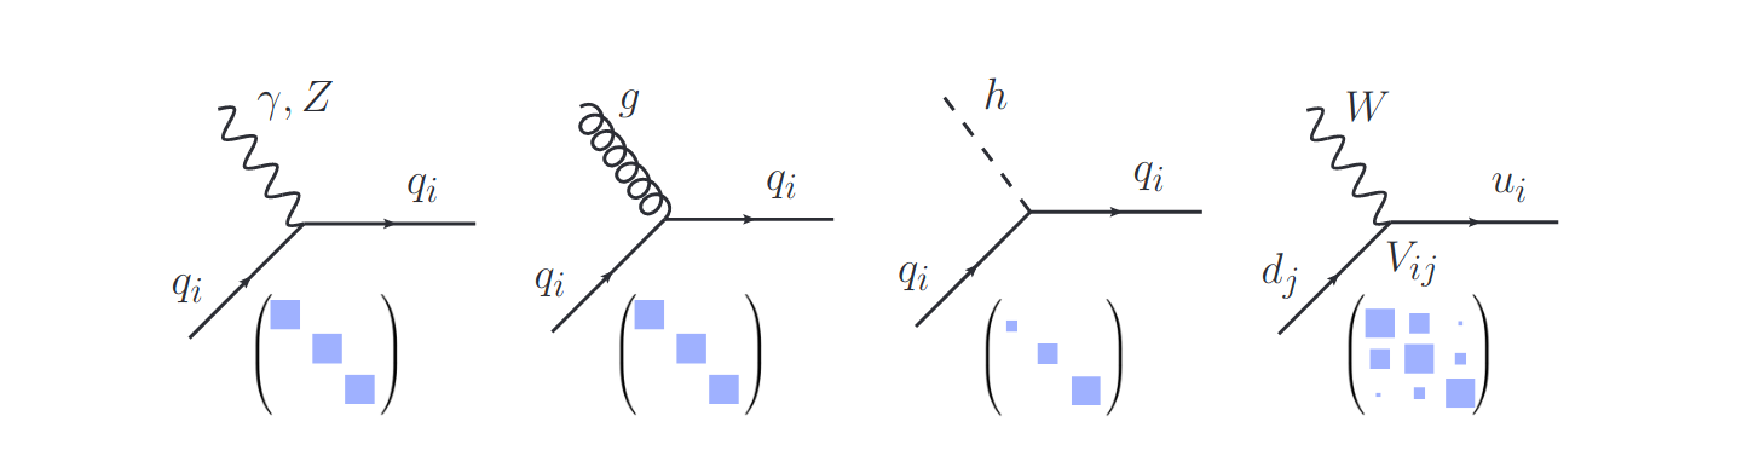
\includegraphics[width=0.9\textwidth]{TestYukawaCouplings.pdf}
	\caption{Feynman diagrams for flavour conserving couplings of quarks to photon, $Z$ boson, gluon and the Higgs (the first three diagrams), and the flavour changing coupling to the $W$ (the last diagram). The $3\times3$ matrices are visual representations of couplings in the generation space, with couplings to $\gamma$ ,$Z$, $g$ being flavour universal, while the couplings to the Higgs are flavour diagonal but not universal. Finally the couplings involving the $W$ are flavour changing and hierarchical.}
	\label{fig:QuarkCKM}
\end{figure}
%´
Note, the CKM matrix elements are fundamental parameters of the particle physics and their precise determination a important landmark for experimental particle physics. It follows then that reproducing the quark mixing parameters is fundamental for BSM searches that include changes to how the quarks interact with possible new Higgs bosons. 
